\documentclass{report}

\usepackage[french]{babel}
\usepackage[T1]{fontenc}
\usepackage[utf8]{inputenc}
\title{Rapport du projet de C/SD}
\author{Nathan BARLOY, Valentin CRÔNE, Johan TOMBRE}
\date{April 10, 2018}
\usepackage{tabularx}
\usepackage{verbatim}
\usepackage{graphicx}
\usepackage{amsmath}
\usepackage{amssymb}
\usepackage{moreverb}
\usepackage{listings}
\usepackage{dsfont}
%\usepackage{fontspec}
\usepackage{hyperref}

\usepackage{algorithm}
\usepackage{algorithmic}
\usepackage{colortbl}
\usepackage{subfiles}
\usepackage{pdfpages}
\begin{document}
\begin{titlepage}
\centering
        \begin{flushleft}\hspace{1cm}
\begin{flushleft}
\includegraphics[keepaspectratio, width=5cm,height=5cm]{img/Logoinp.jpg}\end{flushleft}
        \end{flushleft}
        \vspace*{-4cm}
        \begin{flushright}
        
\includegraphics{img/Logouniv.jpg}
        \end{flushright}
        \vspace*{1cm}
        \vspace*{1cm}
        {\LARGE \bfseries Rapport de projet de C/SD \par}
        \vspace*{0.5cm}
        {\LARGE \bfseries par\par}
        \vspace*{0.5cm}
        {\LARGE \bfseries Nathan BARLOY, Valentin CRÔNE, Johan TOMBRE\par}
        \vfill
        \begin{flushright}
\begin{flushright}
\includegraphics[keepaspectratio, width=5cm,height=5cm]{img/LogoTelecom.png}\end{flushright}
        {\scshape
        1 Avenue Paul Muller\\
        54600 Villers-lès-Nancy\\
        France}
        \end{flushright}
        \vspace*{-1cm}
        \begin{flushleft}
        {\scshape Projet de C/SD}
        \end{flushleft}
\end{titlepage}

\newpage
\tableofcontents
\chapter{État de l'art}
\section{Introduction}
\subsection{Qu'est ce qu'un système de recommandation?}
Un système de recommandation a pour but de fournir des recommandation de résultats pertinentes à un utilisateur, en fonction de différents paramètres comme ses préférences, son historique, le temps passé sur le contenu, etc.., afin de lui proposer directement un contenu ciblé sans efforts de sa part.

Un algorithme de recommandation peut de ce fait être utilisé pour faciliter les recherches de contenus sur un thème donné, ce qui est bénéfique pour l'utilisateur car il aura plus d'informations pertinentes à regarder, et permettre aux gérants de la plateforme de fidéliser la clientèle.\par

Prenons un exemple, un site de e-commerce sur lequel on trouve facile des articles en rapport avec l'article que l'on est en train de consulter rendra plus facile la recherche, et donc aidera le client a trouver rapidement le produit adéquat, ce qui réduira le temps nécessaire à l'achat, et évitera la perte du client.
Un autre exemple est une plateforme de visionnage de vidéos en ligne, qui génère des bénéfices grâce a la publicité, un tel système proposera du contenu ciblé intéressant pour l'utilisateur, qui consultera un plus grand nombre de vidéos sur le site, ce qui permet à la fois de satisfaire l'utilisateur et améliorer la génération de revenus liés à la publicité.
Ces effets sont liés au fait que l'utilisateur reçoit des suggestions pertinentes de la part du système de recommandation auxquelles il n'aurait pas forcément pu prêter attention autrement.\par

\newpage
\subsection{La place des systèmes de recommandation dans la recherche d'information}

La recherche d'information sur internet est fondée sur un principe d'indexation des données. Afin de pouvoir répondre aux requêtes des utilisateurs dans un temps raisonnable, on indexe les données dans une base de données, et on les filtre en fonction de la requête des utilisateurs. Les requêtes sont entrées à partir de mots clés (requêtes ad hoc), et le moteur de recherche va alors retourner les résultats qui correspondent.
Le nombre conséquent de résultats obligera le moteur de recherche a limiter la quantité d'informations retournée en limitant un certain nombre de résultats par page.
Ce système fonctionne plutôt bien, mais nécessite que l'utilisateur traite lui même un grand nombre de résultats, ce qui peut se limiter a la ou les premières pages car il lui est impossible de tout traiter.
On cherche donc à rendre les résultats de la première page plus pertinents. On fait alors immédiatement le lien avec les systèmes de recommandation, car au lieu de filtrer par mots clés, on va pouvoir rechercher des contenus à thème proche, date proche, et personnaliser les résultats en fonction des habitudes de l'utilisateur.\par

Ces exemples montrent un certain nombre de cas où l'utilisation d'un système de recommandation s'avère utile. Cependant il en existe de nombreux autres, car leur champ d'application est immense, c'est pourquoi il est intéressant de s'intéresser aux systèmes existants pour tenter de les reproduire et les améliorer.

%\subsection{Historique}
%A mettre ou pas?

\newpage
\subsection{Classer les différents systèmes de recommandation}
Il existe différents types de systèmes de recommandation, en fonction du type de données à classer, de la puissance disponible, de activités utilisateurs, des besoins de l'entreprise, et de nombreux autres facteurs.
Les facteurs principaux à retenir sont:
\begin{itemize}
	\item La connaissance des préférences utilisateur.
	\item La similarité entre les utilisateurs, les uns par rapport aux autres. (Métrique)
	\item La connaissance d'informations sur des données à recommander
	\item La connaissance d'informations de regroupement sur des données à recommander
\end{itemize}

A partir de ces facteurs on produit différents types de recommandations.
Les systèmes les plus utilisés sont le filtrage basé sur le contenu, et le filtrage collaboratif.

\subsubsection{Le filtrage basé sur le contenu}
Le filtrage basé sur le contenu va essayer d'associer un utilisateur à un ensemble de données proche de ses préférences. On va alors rechercher des données qui pourraient l'intéresser en tenant compte uniquement de lui-même, et de ce qu'il a consulté. Pour cela, il faut dresser des liens entres les différents éléments de la base de donnée, pour pouvoir déterminé si un élément est proche ou non de ce qu'a consulté l'utilisateur.
L'avantage de ce filtrage est qu'il ne nécessite pas d'avoir d'autres utilisateurs pour fonctionner, puisqu'on ne compare pas les utilisateurs entre eux. Cela est donc très pratique quand la base de donnée des utilisateur est petite.
\subsubsection{Le filtrage collaboratif}
Le filtrage collaboratif va mesurer une certaine distance entre un utilisateur donné, et tous les autres utilisateurs pour sélectionner les utilisateurs les plus proches uniquement.
On utilisera alors le profil de ces utilisateurs proches pour regarder les données qui les ont intéressés pour les recommander à notre utilisateur initial.
L'avantage de ce filtrage est qu'il ne nécessite pas de créer un algorithme qui détermine si deux données sont proches ou non. Cependant, si la base de donnée des utilisateurs n'est pas assez fournie, ce filtrage ne sera que très peu efficace.\par
Évidemment, les filtrages les plus efficaces sont ceux qui mélangent les méthodes décrites précédemment, de manière à en tirer les avantages.

\subfile{etat_art/data.tex}
\subfile{etat_art/tf-idf.tex}

\section{La matrice d'usage}
Également appelé le modèle utilisateur, la matrice d'usage contient des données collectées sur les utilisateurs associés aux produits. On le représente généralement sous la forme d'une matrice avec les utilisateurs sur les lignes et les produits en colonne. Les scores attribués peuvent être une note, un nombre de consultation, un durée, un like... Cette matrice comporte généralement de nombreuses valeurs manquantes qu'il va falloir chercher à déterminer grâce à notre système de recommandation.  Il est également intéressant de remarquer que les goûts des utilisateurs évoluent au cours du temps. Il est donc important de réajuster les données de cette matrice régulièrement.
\section{Réduction de matrice}
Reprenons la matrice d'usage tout juste présentée. Elle est de dimension $m.n$ avec m le nombre d'utilisateurs et n le nombre de produits. Dans la pratique, cela représente habituellement des milliers / millions d'utilisateurs pour autant voire plus de produits. On obtient donc une matrice possédant des milliards de valeurs. Il serait donc très long d'effectuer des calculs dessus pour en déduire des recommandations. La solution est donc de réduire la dimension de la matrice.
\vspace{0.5cm}

Plusieurs approches sont possibles. On peut, par exemple, ne pas prendre en compte les utilisateurs dont on ne possède que très peu d'informations ou de la même manière retirer les produits peu populaires et donc ayant moins de chance d'intéresser les utilisateurs. Cependant, cette méthode a comme gros inconvénient de réduire le champ des recommandations proposées. En effet, comment proposer à un utilisateur un produit qui lui conviendrait parfaitement s'il est retiré de la liste car peu connu ? Cela restreint plus ou moins les produits recommandables à ceux qui sont populaires et donc déjà connus par la plupart.\par
Une autre approche consiste à ne conserver qu'une gamme de produits répondant à un critère spécifié. Par exemple, il est possible de supprimer les films de genre romantique si l'utilisateur ne manifeste aucun intérêt pour ce genre. Enfin, une dernière méthode consiste à ne prendre en compte que les utilisateurs jugés comme étant proche de l'utilisateur cible, c'est ce qu'on appelle le clustering (détaillé dans la section suivante).\par
L'avantage de cette méthode est donc de réduire le temps de calcul pour déterminer une recommandation. Cependant, la qualité de la recommandation s'en retrouve impactée. En effet cela réduit le nombre de personnes analysés par l’algorithme dans le cas d’une réduction du nombre d’utilisateur, et une réduction du nombre de produits réduira le champs des recommandations à un certains type.

\subfile{etat_art/clustering.tex}
\subfile{etat_art/similarite.tex}



\chapter{Rapport}

\section{Introduction}
Le but de ce projet est de concevoir un système de recommandation comme le propose Netflix, Google (Youtube), Amazon et beaucoup d'autres pour la recommandation de leurs produits.\par
Au cours de ce rapport, nous aborderons les choix que nous avons pris tout au long de ce projet, la présentation du code réalisé, le choix des structures ainsi que l'analyse des résultats obtenus.

\subfile{bdplus/bdplus.tex}

\section{Création d'une distance entre les films}
Chaque film est caractérisé par la donnée de différents attributs. Dans le cas présent, les attributs que nous considérerons sont :
\begin{itemize}
    \item L'année de parution
    \item Les acteurs
    \item Le réalisateur
    \item Le genre
    \item Le type (film ou série)
\end{itemize}
Pour chacun de ces attributs, on va calculer une distance, dont la valeur sera comprise entre 0 et 1 (0 pour identique, et 1 pour complètement différent). On fait ensuite simplement une moyenne pondérée des distances obtenues. Les poids de cette moyenne sont modulables, ce qui nous permet de les modifier comme on le souhaite, pour avoir des proportions qui correspondent à ce que nous voulons.\\
Cette distance doit vérifier certaines propriétés de la distance mathématique :
\begin{itemize}
    \item \(d(a,b)=d(b,a)\) (la symétrie)
    \item \(d(a,b) \geq 0\) (la positivité)
    \item \(d(a,a)=0\)
\end{itemize}
Si la distance créée ne vérifie pas ces propriétés, alors elle n'est pas bonne.

\subsection{La distance de Jacard}
En mathématique, la distance entre 2 ensembles est souvent calculée comme étant le minimum des distances entre les points de ces ensembles :
\[d(E,F)=\min_{\substack{x\in E \\ y\in F}} d(x,y)\]
Cependant, dans notre cas, cette distance n'est pas très utile, puisqu'elle ne prend pas en compte les autres éléments des ensembles. Ainsi, une telle distance ne ferrais pas de différence entre 2 films où tous les acteurs sont les mêmes, et 2 films qui ont  un seul acteur en commun. Il faut donc trouver autre chose : la distance de Jacard.\par
Cette distance permet de mesurer la similarité entre 2 ensembles finis : soient $X$ et $Y$ deux ensembles finis. Alors,
\[dist\_Jacard=1-\frac{|X \cap Y|}{|X \cup Y|}\]
On a bien que si \(X=Y\), alors la distance de Jacard est nulle, et que si les deux ensembles sont complètement distincts, alors la distance vaut 1.\\
Cependant, on peut se dispenser de certains calculs pour trouver la distance de Jacard. En effet, on peut utiliser le fait que \(|X \cup Y|=|X|+|Y|-|X \cap Y|\). Il n'y a alors plus qu'a calculer \(|X \cap Y|\) pour pouvoir ensuite calculer la distance de Jacard.\par
Cette distance de Jacard pourra être utilisée pour calculer les distance entre les attributs des films qui sont des ensembles. Dans notre cas, cela représente les acteurs, les réalisateurs et les genres.\\
Après quelques tests, on se rend compte que même si l'algorithme marche la plupart du temps, il y a certains cas ou il plante à l'exécution et indique une division par zéro. Après quelques recherches, on comprend que cela est du au fait que parfois, la liste des acteurs, des réalisateurs ou des genres est vide. Ainsi, la distance de Jacard ne peut pas être calculée, puisqu'on divise par \(|X \cup Y|\), qui vaut zéro si $X$ et $Y$ sont vides.\par
Ce bug nous permet aussi de nous rendre compte de l'absurdité de certains calculs : en effet, comment interpréter la distance entre en ensemble vide est un autre ensemble qui ne l'est pas forcement ? (par exemple, si on sait uniquement que le réalisateur du film 1 est Spielberg, et rien pour le film 2) Dans ce cas, donner une distance n'a aucun sens. Il faut donc aussi prendre en compte cela avant de faire les calculs.\par
Après quelques tests, on se rend compte que l'on obtient parfois une distance négative, ce qui est impossible pour une distance normalement : il y a donc un problème dans le code. Il se trouve en fait qu'il y avait un problème au niveau de certains types, ce qui faussait la fonction equals, qui sert a comparer 2 éléments entre eux. Après correction, on obtient quelque chose de cohérent. Notamment, la distance entre un film et lui-même est toujours 0.\par
Cette distance de Jacard permet de donner une distance entre 2 ensembles : on peut donc l'utiliser pour tous les attributs qui sont des listes, i.e. les acteurs, les réalisateurs, et les genres.

\subsection{La distance entre les années}
Pour créer une distance entre 2 années, on va bien évidemment considérer la distance entre ces 2 entiers : cela signifie prendre la valeur absolue de la différence (\(|a1-a2|\)). Notre distance sera donc une fonction $f$ qui sera à valeur dans $\mathds{R}_{+}$. On va chercher des conditions sur cette fonction.\par
Tout d'abord, on veut obtenir une distance entre 0 et 1, donc doit aller de $\mathds{R}_{+}$ dans \([0;1]\). De plus, on veut que l'ordre soit gardé : si \(a>b\), on veut que \(f(a)>f(b)\). Cela signifie que la fonction est croissante. Enfin, on doit avoir que $f(0)=0$ et $\lim\limits_{x \rightarrow +\infty} f(x)=1$.\par
En résumé, on cherche une fonction croissante de $\mathds{R}_{+}$ dans $[0;1]$ qui atteint ses bornes.\par
une première fonction à laquelle on peut penser est une fonction que l'on rencontre souvent en physique :
\[f(x)=1-e^{-\frac{x}{\tau}} , \tau \in \mathds{R}_{+}^{*}\]
On peut alors faire varier le paramètre $\tau$ pour moduler la fonction comme on veut. La valeur que nous avons choisi est $\tau=10$, car on a alors que pour avoir une distance de 0.5, il que les deux dates soient séparées de 7 ans, ce qui correspond à peu près à ce qu'on veut.\par
Une autre fonction utilisable possible est la fonction arctangente. On a alors
\[f(x)=\arctan(\alpha \cdot x)\times \frac{2}{\pi} , \alpha \in \mathds{R}_{+}^{*}\]
Comme précédemment, on cherche une valeur du paramètre $\alpha$ qui corresponde à nos attentes. Dans ce cas, on prend $\alpha=0.15$, ce qui donne une distance de 0.5 pour 7 années d'écart.\par
Dans tous les cas, c'est une bonne chose d'avoir des paramètres modifiables dans ces fonctions pour pouvoir mieux approcher ce que l'on veut.
\subsection{Amélioration de la distance entre les genres}
Pour la distance entre les genres, on utilisait jusqu'à présent la distance de Jacard. C'est une méthode qui marche, mais elle omet certains éléments dans son calcul, ce qui le rend moins précis. En effet, on ne prend pas en compte les potentielles ressemblances entre genres, on regarde simplement si un même genre est présent dans les deux films. Ainsi, si l'on considère 3 films dont les genres sont respectivement crime, mystère et romance, la distance de Jacard entre ces 3 films sera nulle, et on ne pourra pas les classer. Cependant, on se rend bien compte que les genres crime et mystère sont proches, alors qu'ils ne le sont pas de romance. Il faut donc essayer de prendre en compte les distances intrinsèques entre deux genres.\par
Pour cela, la meilleure méthode aurait été d'utiliser le machine learning. Avec une telle méthode, l'humain n'a pas besoin d'intervenir, il suffit d'analyser la base de donnée des films et de repérer ceux qui sont proches d'après les utilisateurs pour estimer des distances entre les genres. L'avantage est que l'on peut alors rajouter un nouveau genre sans problème, et sans expliciter son lien avec les autres genres : l'algorithme fait cela tout seul. Cependant, pour qu'une telle méthode marche, il faut une base de données assez conséquente pour avoir des résultats corrects. De plus, c'est une méthode difficile à mettre en place, et qui requiert des connaissances que nous n'avons pas.\par
Il faut donc utiliser une autre méthode, plus fastidieuse et moins précise. On va pour cela créer nous-même une matrice contenant les distances entre les films, puis on fera une moyenne des distances entre les genres du premier film avec ceux du deuxième film. Pour cela, il faut d'abord lister les films existant, qu'on obtient grâce à un simple algorithme qui parcours tous les film. On obtient la liste suivante : Action, Thriller, Drama, Adventure, Family, Romance, Fantasy, Sci-Fi, Animation, Comedy, Horror, Crime, Mystery, History, Musical, Sport, Biography, War et Music; soit un total de 19 genres. On crée ensuite une matrice de distances qu'on utilisera pour nos calculs :
\setcounter{MaxMatrixCols}{20}
\small
$$
\begin{pmatrix}
0.0 & 0.3 & 0.5 & 0.1 & 0.6 & 0.9 & 0.2 & 0.2 & 0.7 & 0.7 & 0.4 & 0.6 & 0.6 & 0.7 & 0.9 & 0.5 & 0.8 & 0.2 & 0.9 \\
0.3 & 0.0 & 0.3 & 0.4 & 0.7 & 0.9 & 0.5 & 0.4 & 0.8 & 0.8 & 0.1 & 0.2 & 0.3 & 0.6 & 0.9 & 0.9 & 0.8 & 0.5 & 0.9 \\
0.5 & 0.3 & 0.0 & 0.6 & 0.7 & 0.4 & 0.5 & 0.6 & 0.8 & 0.8 & 0.3 & 0.3 & 0.3 & 0.2 & 0.4 & 0.6 & 0.5 & 0.6 & 0.8 \\
0.1 & 0.4 & 0.6 & 0.0 & 0.2 & 0.4 & 0.1 & 0.3 & 0.4 & 0.3 & 0.7 & 0.8 & 0.4 & 0.7 & 0.8 & 0.5 & 0.8 & 0.3 & 0.9 \\
0.6 & 0.7 & 0.7 & 0.2 & 0.0 & 0.7 & 0.5 & 0.6 & 0.2 & 0.1 & 0.8 & 0.7 & 0.5 & 0.8 & 0.3 & 0.4 & 0.9 & 0.7 & 0.6 \\
0.9 & 0.9 & 0.4 & 0.4 & 0.7 & 0.0 & 0.7 & 0.8 & 0.7 & 0.5 & 0.9 & 0.8 & 0.6 & 0.4 & 0.1 & 0.6 & 0.6 & 0.5 & 0.3 \\
0.2 & 0.5 & 0.5 & 0.1 & 0.5 & 0.7 & 0.0 & 0.3 & 0.5 & 0.4 & 0.5 & 0.7 & 0.4 & 0.8 & 0.7 & 0.9 & 0.9 & 0.2 & 0.8 \\
0.2 & 0.4 & 0.6 & 0.3 & 0.6 & 0.8 & 0.3 & 0.0 & 0.7 & 0.4 & 0.5 & 0.4 & 0.2 & 0.8 & 0.7 & 0.9 & 0.9 & 0.6 & 0.8 \\
0.7 & 0.8 & 0.8 & 0.4 & 0.2 & 0.7 & 0.5 & 0.7 & 0.0 & 0.1 & 0.7 & 0.7 & 0.4 & 0.8 & 0.3 & 0.8 & 0.9 & 0.7 & 0.4 \\
0.7 & 0.8 & 0.8 & 0.3 & 0.1 & 0.5 & 0.4 & 0.4 & 0.1 & 0.0 & 0.8 & 0.8 & 0.4 & 0.9 & 0.3 & 0.5 & 0.7 & 0.9 & 0.6 \\
0.4 & 0.1 & 0.3 & 0.7 & 0.8 & 0.9 & 0.5 & 0.5 & 0.7 & 0.8 & 0.0 & 0.2 & 0.4 & 0.6 & 0.9 & 0.9 & 0.8 & 0.3 & 0.8 \\
0.6 & 0.2 & 0.3 & 0.8 & 0.7 & 0.8 & 0.7 & 0.4 & 0.7 & 0.8 & 0.2 & 0.0 & 0.1 & 0.3 & 0.8 & 0.9 & 0.7 & 0.3 & 0.9 \\
0.6 & 0.3 & 0.3 & 0.4 & 0.5 & 0.6 & 0.4 & 0.2 & 0.4 & 0.4 & 0.4 & 0.1 & 0.0 & 0.4 & 0.6 & 0.6 & 0.7 & 0.5 & 0.8 \\
0.7 & 0.6 & 0.2 & 0.7 & 0.8 & 0.4 & 0.8 & 0.8 & 0.8 & 0.9 & 0.6 & 0.3 & 0.4 & 0.0 & 0.7 & 0.6 & 0.1 & 0.2 & 0.8 \\
0.9 & 0.9 & 0.4 & 0.8 & 0.3 & 0.1 & 0.7 & 0.7 & 0.3 & 0.3 & 0.9 & 0.8 & 0.6 & 0.7 & 0.0 & 0.6 & 0.8 & 0.6 & 0.1 \\
0.5 & 0.9 & 0.6 & 0.5 & 0.4 & 0.6 & 0.9 & 0.9 & 0.8 & 0.5 & 0.9 & 0.9 & 0.6 & 0.6 & 0.6 & 0.0 & 0.7 & 0.9 & 0.9 \\
0.8 & 0.8 & 0.5 & 0.8 & 0.9 & 0.6 & 0.9 & 0.9 & 0.9 & 0.7 & 0.8 & 0.7 & 0.7 & 0.1 & 0.8 & 0.7 & 0.0 & 0.7 & 0.9 \\
0.2 & 0.5 & 0.6 & 0.3 & 0.7 & 0.5 & 0.2 & 0.6 & 0.7 & 0.9 & 0.3 & 0.3 & 0.5 & 0.2 & 0.6 & 0.9 & 0.7 & 0.0 & 0.8 \\
0.9 & 0.9 & 0.8 & 0.9 & 0.6 & 0.3 & 0.8 & 0.8 & 0.4 & 0.6 & 0.8 & 0.9 & 0.8 & 0.8 & 0.1 & 0.9 & 0.9 & 0.8 & 0.0
\end{pmatrix}
$$
\normalsize
C'est assez indigeste et laborieux à créer, mais une fois cela fait, l'utilisation est très simple. Chaque ligne et chaque colonne correspond à un genre, dans l'ordre de la liste, et à la ligne i colonne j, on a la distance entre le genre i et le genre j. Les propriétés de la distance nous donne alors aussi des propriétés sur la matrice : puisqu'une distance est symétrique (\(d(a,b)=d(b,a)\)), la matrice l'est aussi. De plus la distance entre un genre et lui même est nul, donc les éléments diagonaux sont tous nuls.\par
Pour créer notre distance entre 2 ensembles de genres, on va simplement parcourir les 2 ensembles, et faire la moyenne de toutes les distances que l'on trouve grâce à notre matrice. Ainsi, si le film 1 a $n$ genres et le film 2 en a $m$, on va faire la moyenne de $m\times n$ distances entre genres.\par
Il y a cependant un inconvénient à cet algorithme : il donne toujours des distances assez basses, même s'il permet de mieux ordonner. En effet on peut constater que la distance entre 2 ensembles identiques ne vaut pas toujours 0, ce qui peux poser certains problèmes.

\subsection{Recommandation de contenu}
Une fois qu'on a une méthode qui nous calcule une distance entre 2 films, on peut facilement créer une méthode qui prend en argument un film, et qui nous en recommande d'autres. Il suffit pour cela de calculer la distance entre ce film et chacun des autres, puis de trier par ordre décroissant. Les premiers films de la liste sont alors ceux à recommander.

\subfile{collab_rec/collab_rec.tex}
\subfile{sd/sd.tex}
\subfile{sd/static.tex}
\subfile{sd/dynamic.tex}
\subfile{fct/fct.tex}
\subfile{fct/server.tex}
\subfile{fct/cli.tex}
\subfile{fct/gui.tex}
\subfile{network/network.tex}

\subfile{duree/duree.tex}

\subfile{gdp/gdp.tex}

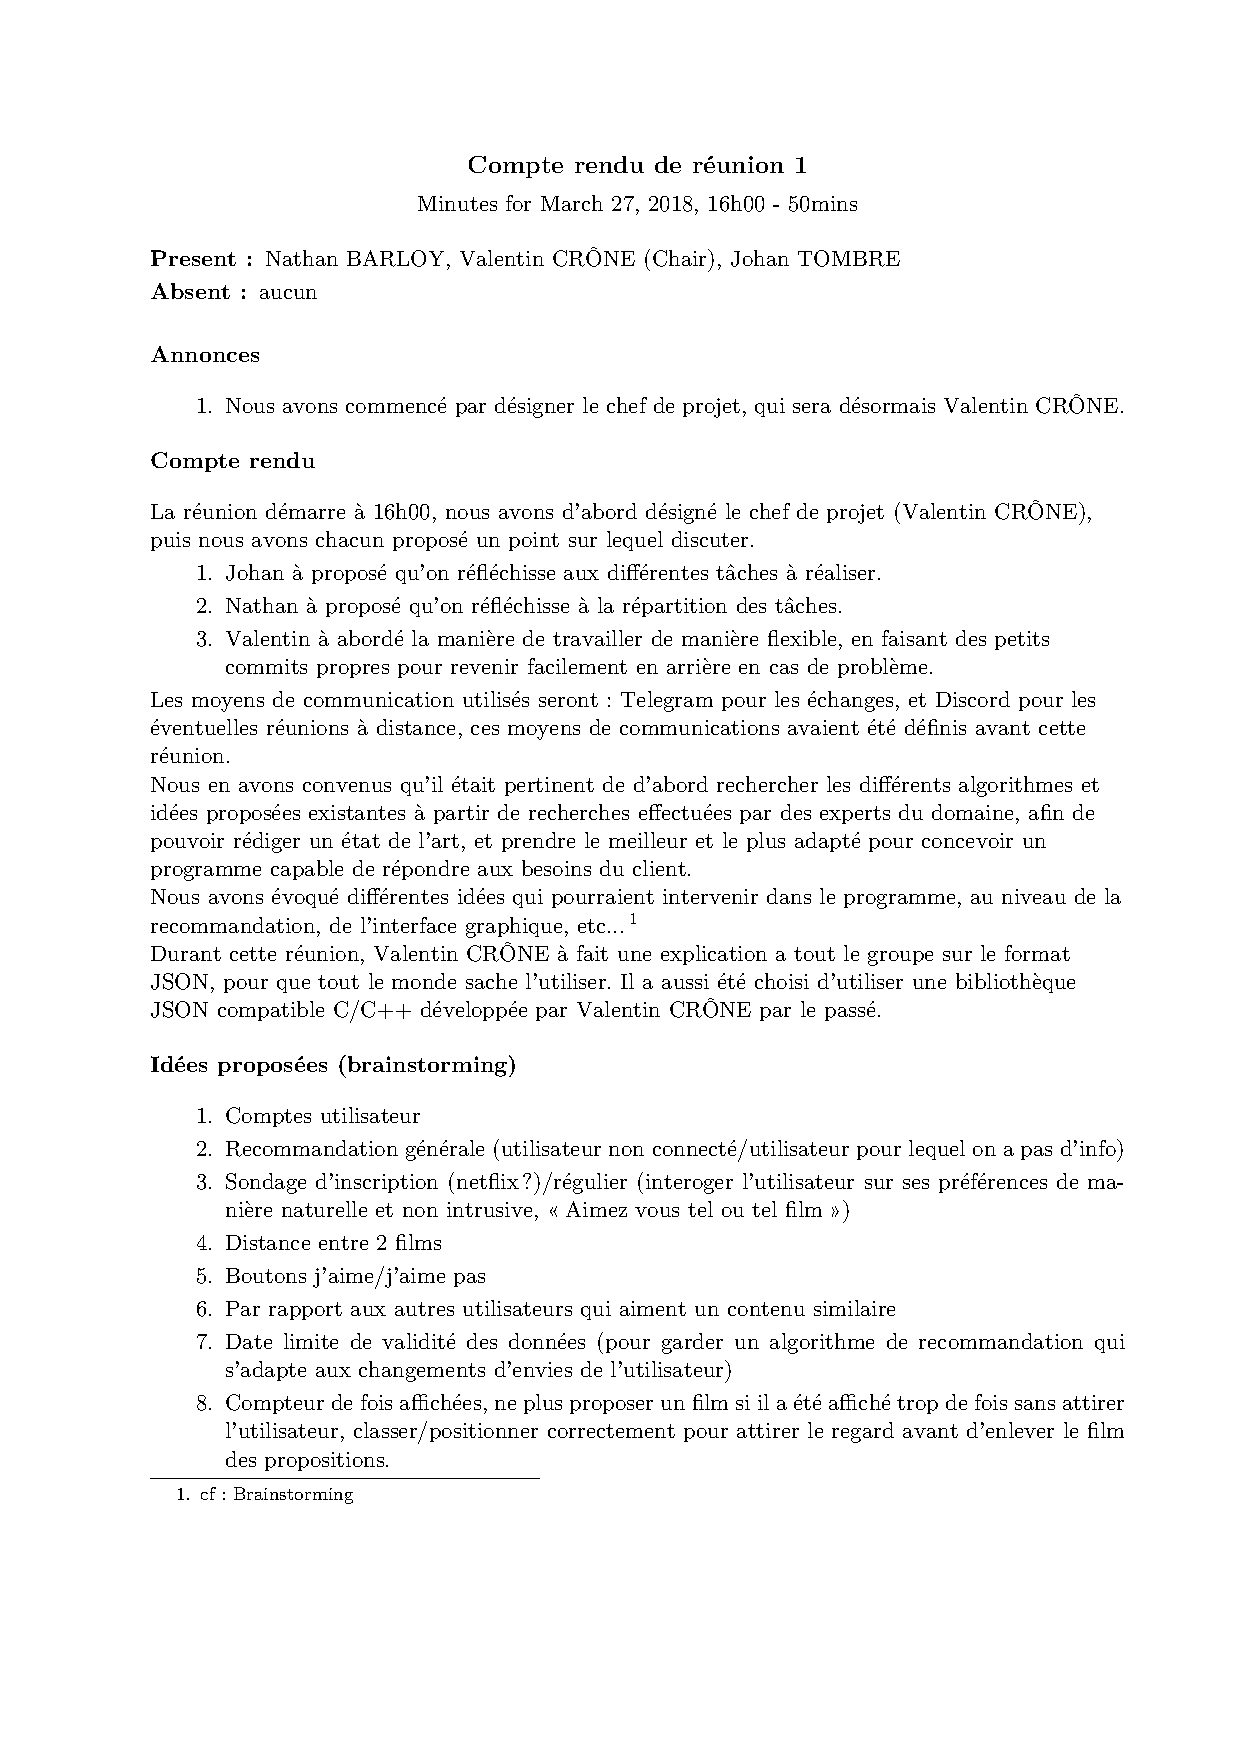
\includepdf[pages=-]{../Reunion/latex/2018-03-27_Reunion_1.pdf}
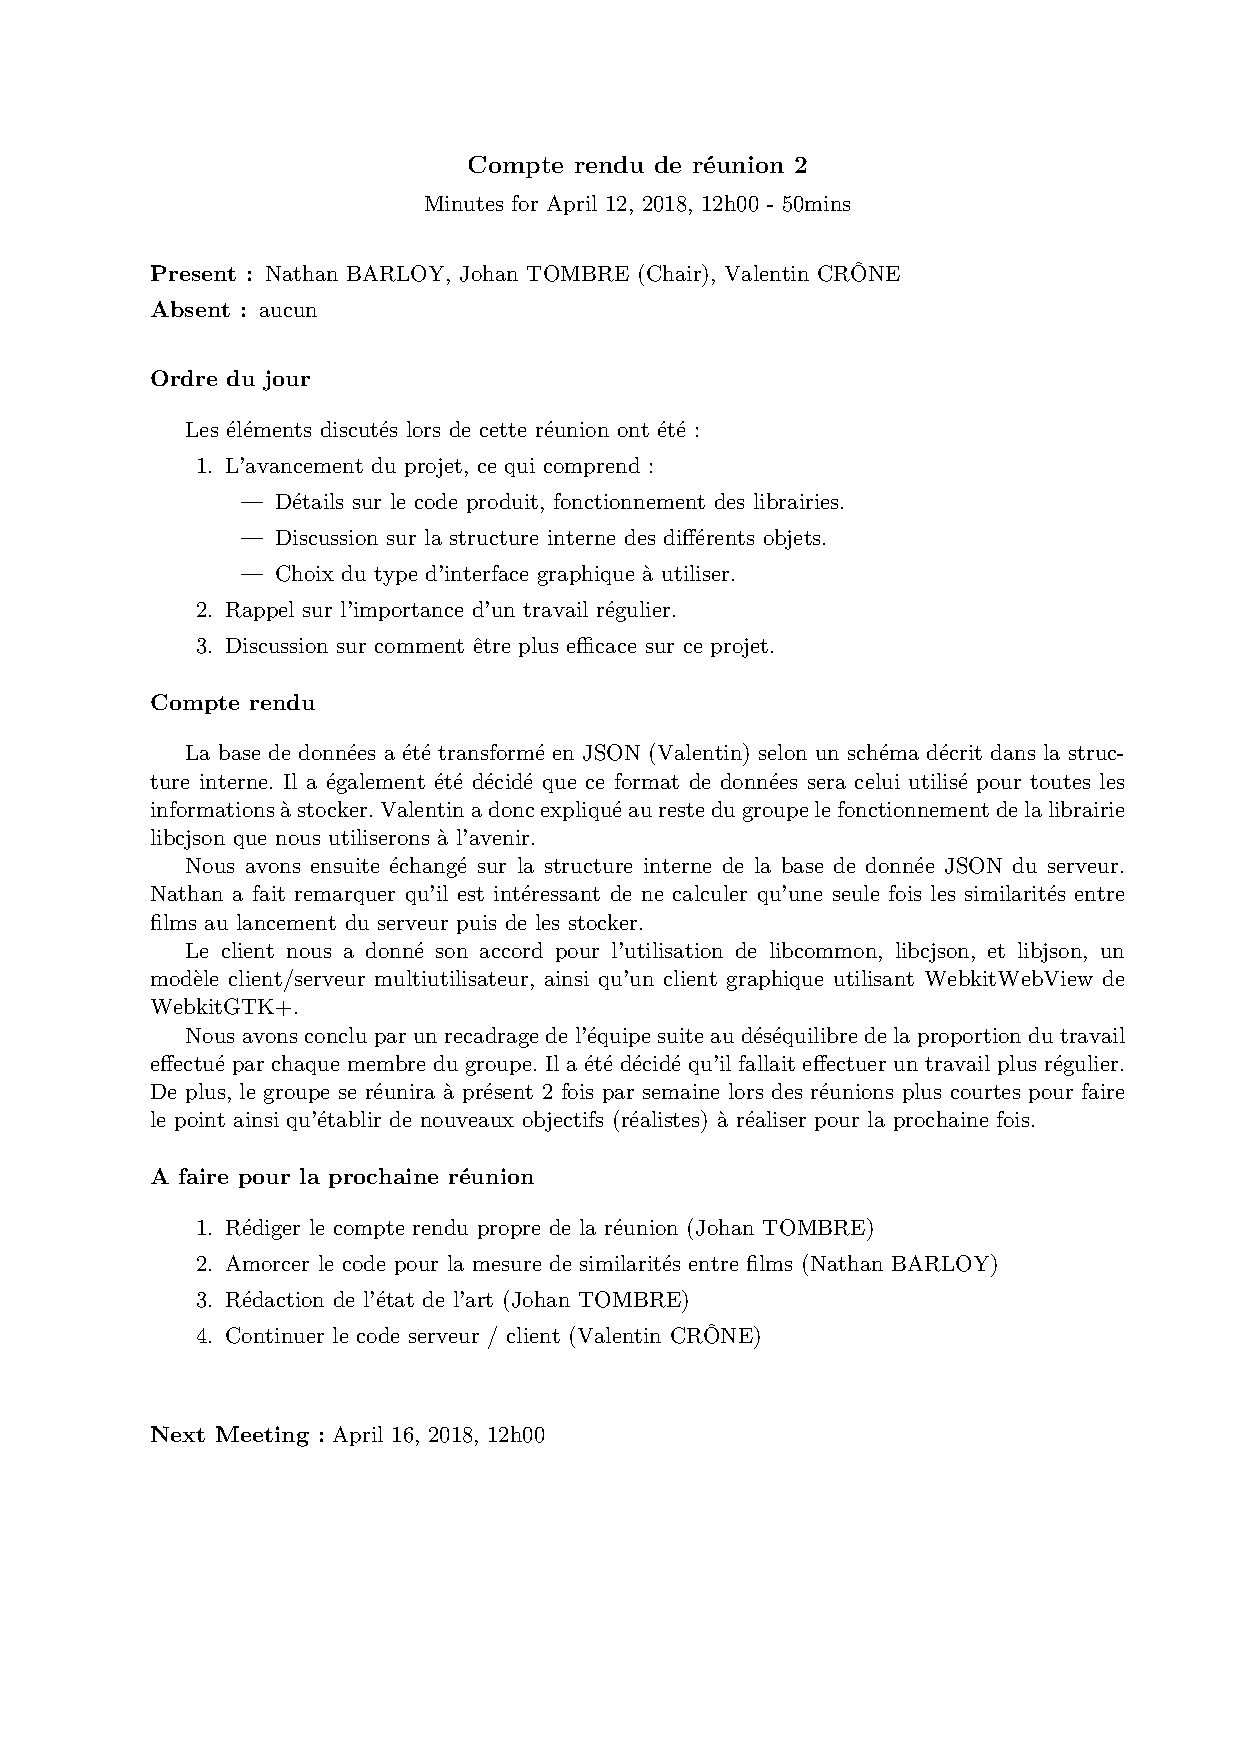
\includepdf[pages=-]{../Reunion/latex/2018-04-12_Reunion_2.pdf}
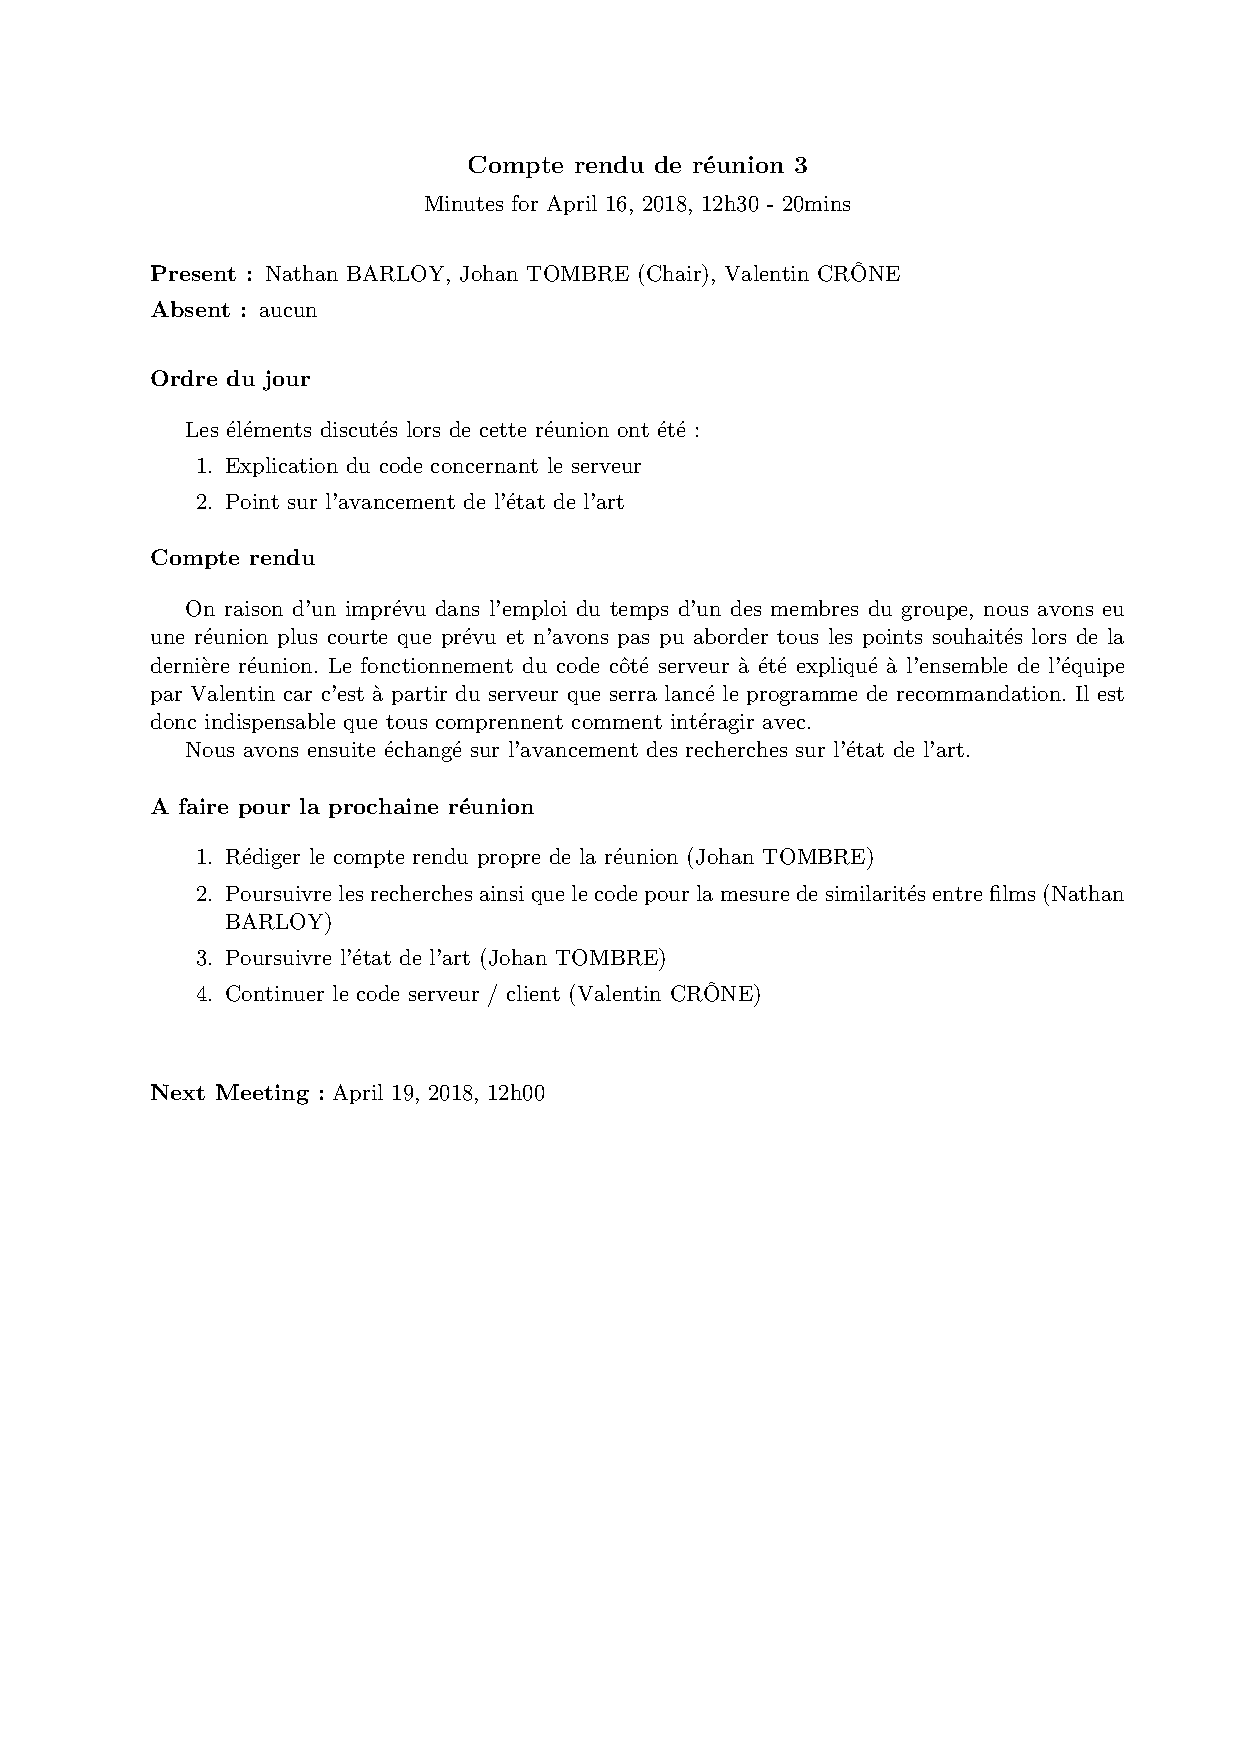
\includepdf[pages=-]{../Reunion/latex/2018-04-16_Reunion_3.pdf}
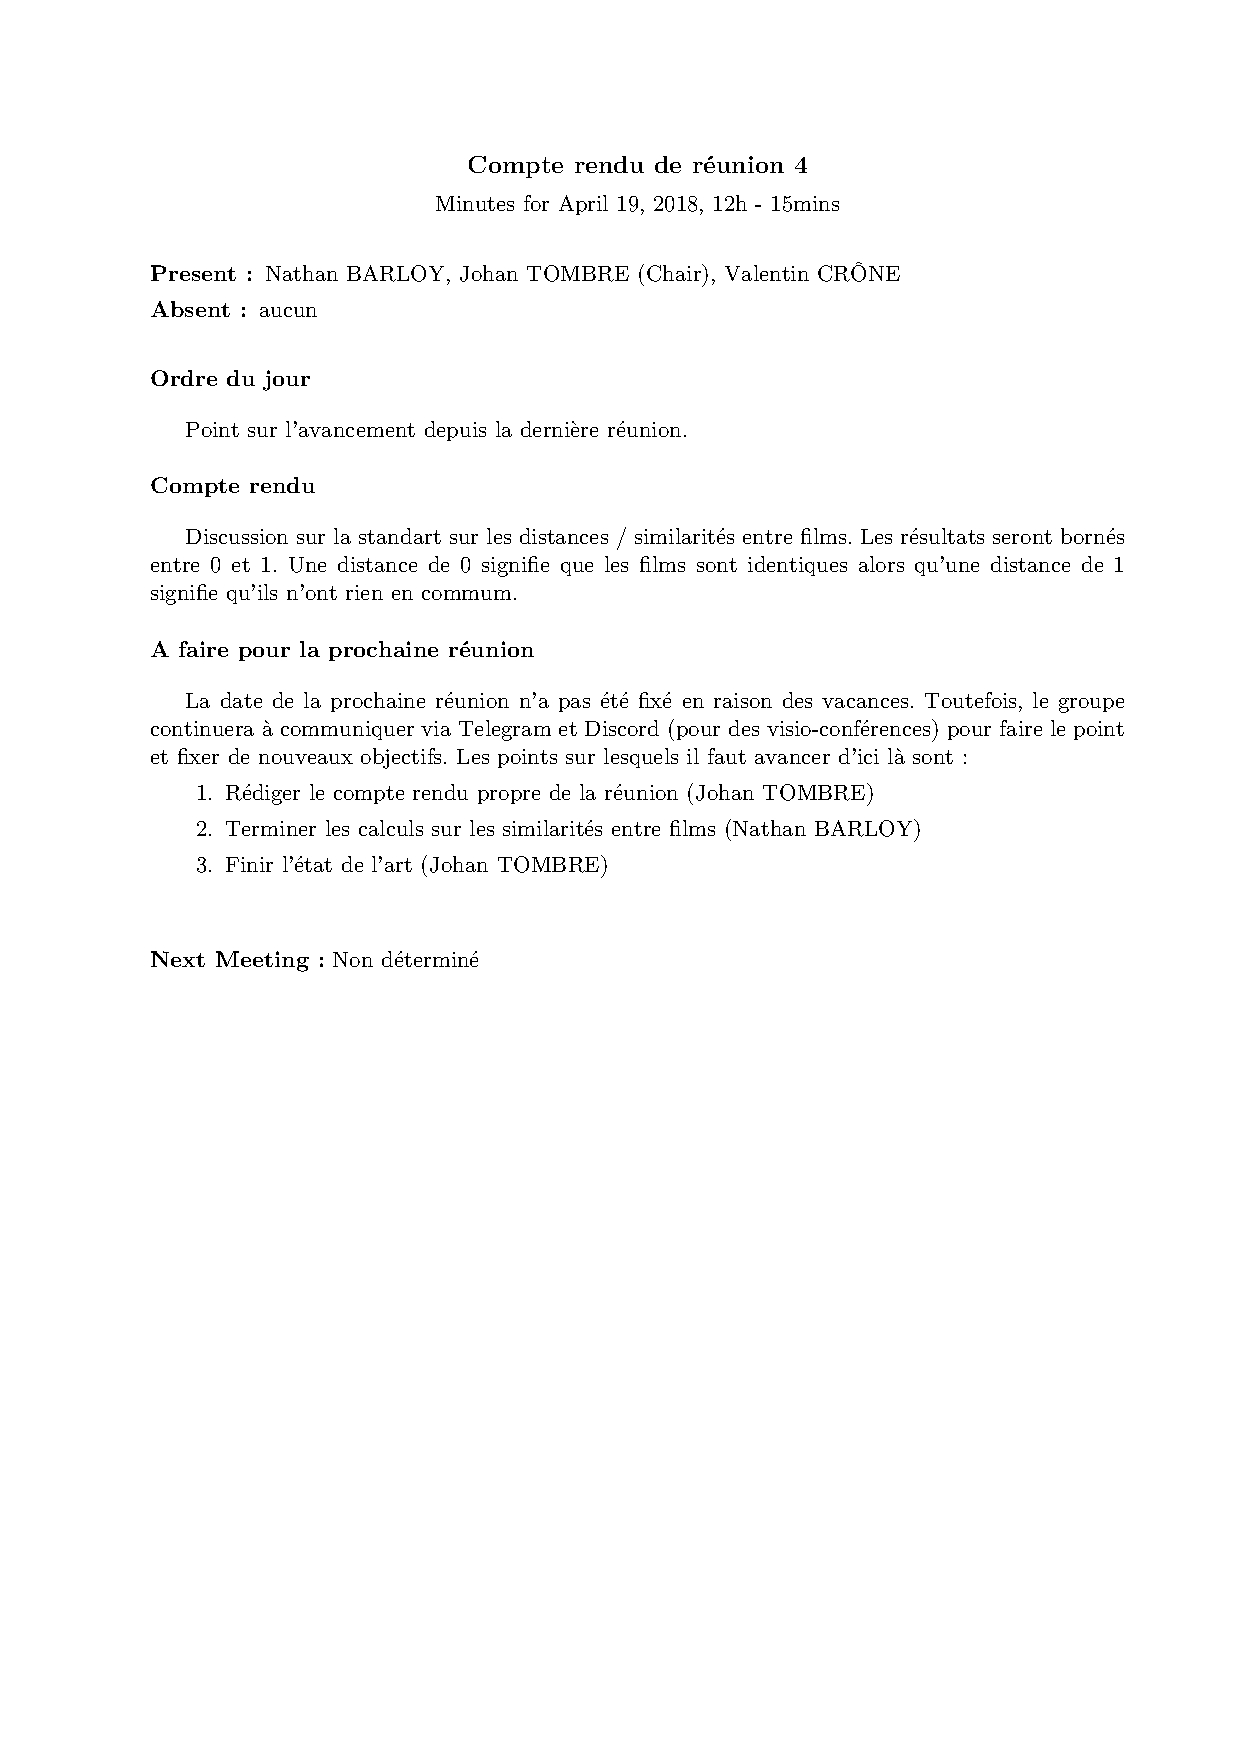
\includepdf[pages=-]{../Reunion/latex/2018-04-19_Reunion_4.pdf}
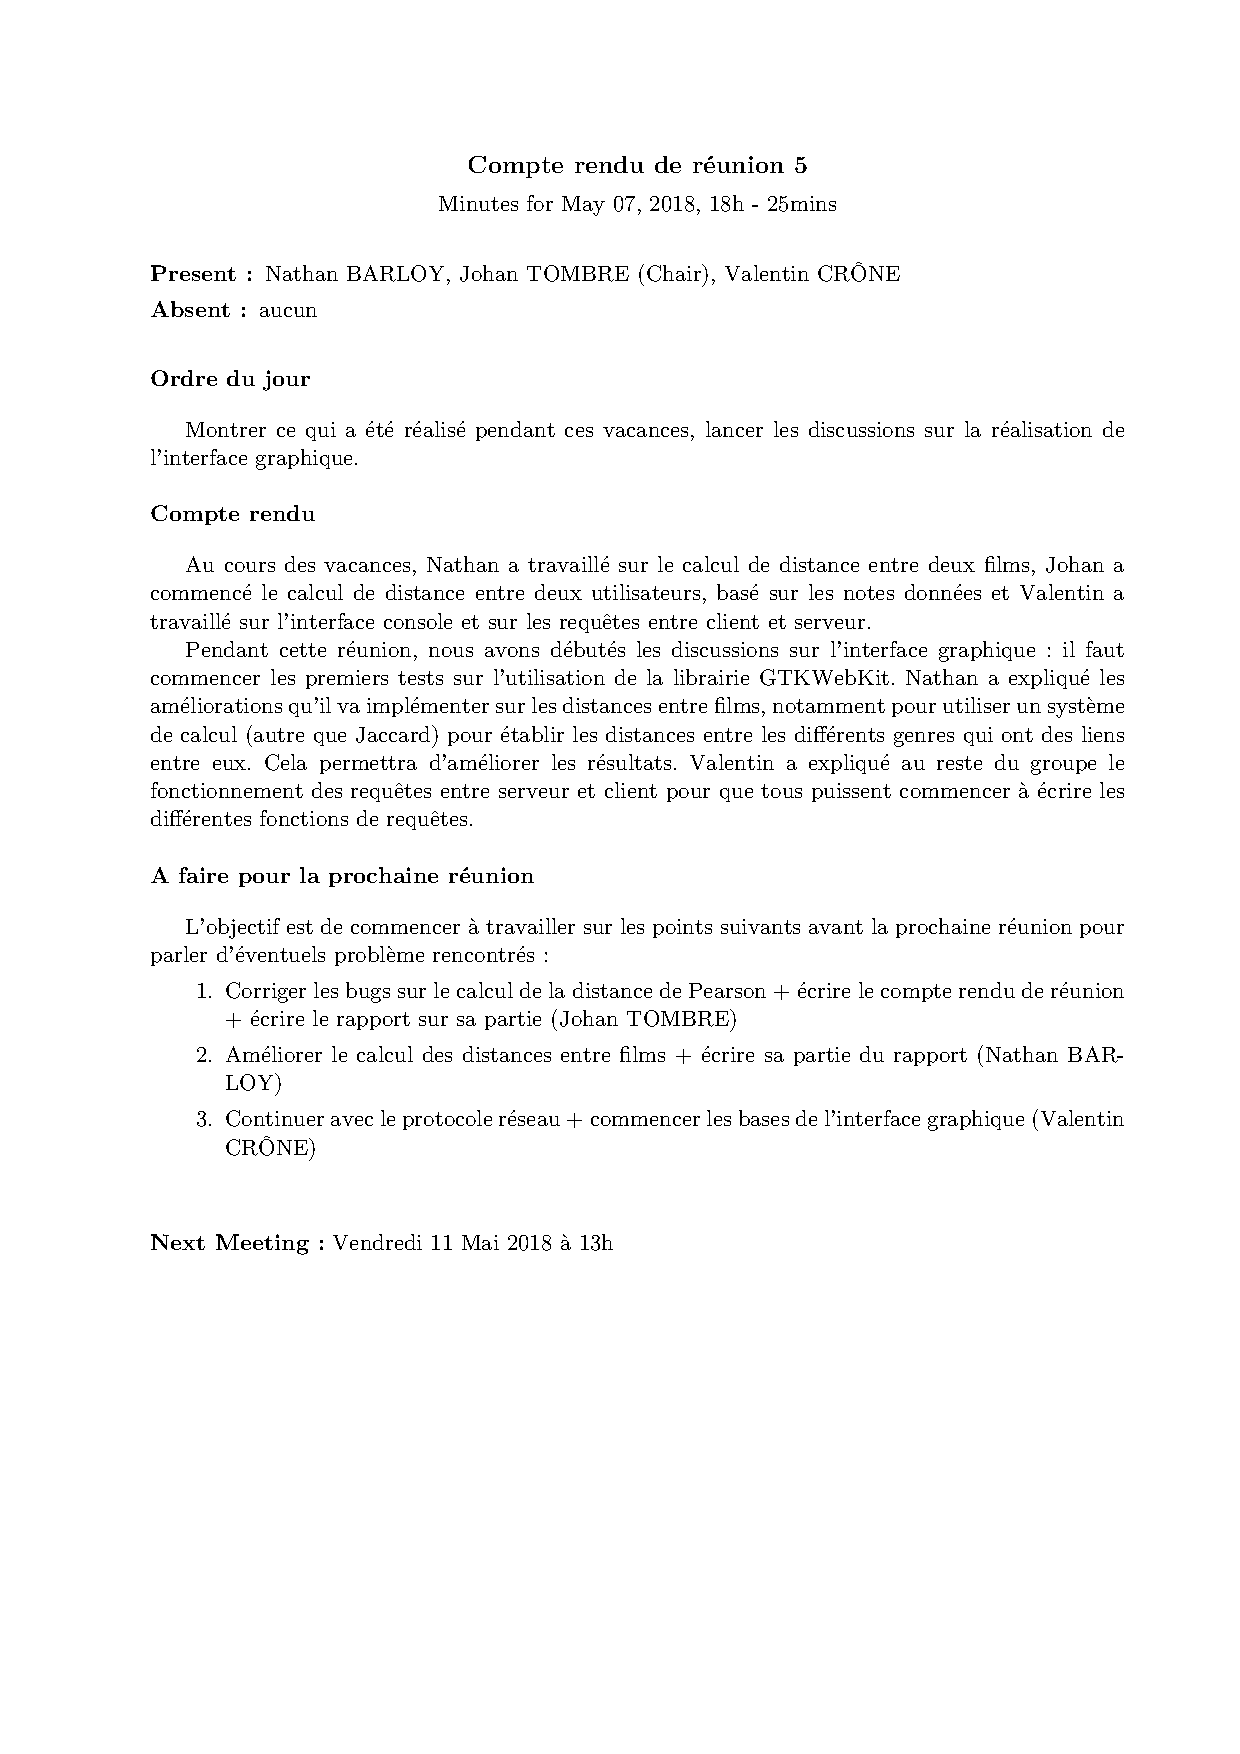
\includepdf[pages=-]{../Reunion/latex/2018-05-07_Reunion_5.pdf}


\end{document}
